\documentclass{beamer}
\usetheme{Madrid}
\usecolortheme{beaver}
\usepackage{tikz}
\usepackage{amsmath}
\usepackage{amssymb}

\title{Causal Reasoning: From Mill to Modern Experiments}
\author{Brendan Shea, PhD}
\date{Introduction to Logic}


\begin{document}

\begin{frame}
    \titlepage
\end{frame}

\begin{frame}{What Does It Mean When We Say 'A Causes B'?}
    \begin{itemize}
        \item When we say "A causes B," we mean that A makes B happen in some way.
        \item A causal relationship implies that if we change A, B will also change as a result.
        \item \textbf{Causality} refers to the relationship between events where one event (the cause) brings about another event (the effect).
        \item Understanding causality helps us explain why things happen and predict what might happen in the future.
    \end{itemize}
    
    \begin{block}{Key Question}
        How can we be sure that A really causes B, and it's not just coincidence or something else causing both A and B?
    \end{block}
\end{frame}

\begin{frame}{Correlation vs. Causation: Why They're Not the Same}
    \begin{itemize}
        \item \textbf{Correlation} means two things tend to happen together or change together.
        \item \textbf{Causation} means one thing actually makes the other thing happen.
        \item Just because two things happen together doesn't mean one causes the other.
        \item Both events might be caused by a third factor we haven't considered.
    \end{itemize}
    
    \begin{center}
    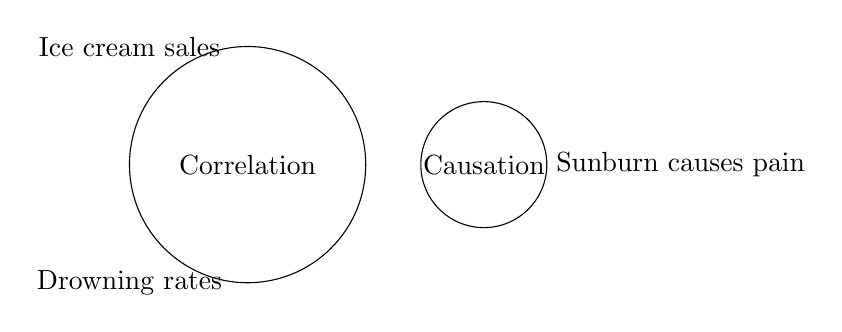
\begin{tikzpicture}
        % Correlation circle
        \draw (0,0) circle (1.5cm);
        \node at (0,0) {Correlation};
        
        % Causation circle
        \draw (3,0) circle (0.8cm);
        \node at (3,0) {Causation};
        
        % Labels
        \node at (-1.5,1.5) {Ice cream sales};
        \node at (-1.5,-1.5) {Drowning rates};
        \node at (5.5,0) {Sunburn causes pain};
    \end{tikzpicture}
    \end{center}
\end{frame}

\begin{frame}{The History of Causal Reasoning: From Aristotle to Today}
    \begin{itemize}
        \item Aristotle (384-322 BCE) identified four types of causes: material, formal, efficient, and final causes.
        \item David Hume (1711-1776) questioned whether we can truly observe causation or just regular succession of events.
        \item John Stuart Mill (1806-1873) developed systematic methods for establishing causal relationships.
        \item Modern scientists use statistical methods and controlled experiments to determine causality.
    \end{itemize}
    
    \begin{alertblock}{Important Development}
        The shift from philosophical reasoning to empirical scientific methods has been crucial for establishing reliable causal relationships.
    \end{alertblock}
\end{frame}

\begin{frame}{John Stuart Mill and the Quest for Causality}
    \begin{itemize}
        \item John Stuart Mill was a British philosopher who systematized approaches to find causal relationships.
        \item Mill's work "A System of Logic" (1843) formalized methods for scientific inquiry.
        \item Mill believed that careful observation and comparison could reveal causal connections.
        \item His methods remain influential in scientific reasoning and experimental design today.
    \end{itemize}
    
    \begin{example}
        Mill was concerned with questions like: "Does this medicine cure this disease?" or "Does this educational technique improve learning?"
    \end{example}
\end{frame}

\begin{frame}{Introduction to Mill's Methods: Five Ways to Find Causes}
    \begin{itemize}
        \item Mill developed five systematic methods to identify causal relationships through observation.
        \item These methods provide a framework for thinking about what causes what.
        \item Mill's methods help us differentiate between coincidence and true causation.
        \item These techniques form the foundation of modern experimental design.
    \end{itemize}
    
    \begin{block}{Mill's Five Methods}
        \begin{enumerate}
            \item Method of Agreement
            \item Method of Difference
            \item Joint Method of Agreement and Difference
            \item Method of Residues
            \item Method of Concomitant Variation
        \end{enumerate}
    \end{block}
\end{frame}

\begin{frame}{Method of Agreement: Finding What's Common When Effects Are Similar}
    \begin{itemize}
        \item The \textbf{Method of Agreement} looks for the one factor that is present in all cases where the effect occurs.
        \item If multiple instances of a phenomenon have only one circumstance in common, that circumstance is likely the cause.
        \item This method works by examining different scenarios that produce the same effect.
        \item It helps identify necessary conditions for an effect to occur.
    \end{itemize}
    
    \begin{table}
        \centering
        \begin{tabular}{|c|c|c|c|c|}
            \hline
            \textbf{Case} & \textbf{Factor A} & \textbf{Factor B} & \textbf{Factor C} & \textbf{Effect X} \\
            \hline
            1 & Present & Present & Absent & Occurs \\
            2 & Present & Absent & Present & Occurs \\
            3 & Present & Absent & Absent & Occurs \\
            \hline
            \multicolumn{5}{|c|}{Factor A is likely the cause of Effect X} \\
            \hline
        \end{tabular}
    \end{table}
\end{frame}

\begin{frame}{Method of Agreement Example: Professor Frink's Lab Explosion}
	\textbf{Scenario:} Professor Frink is investigating what causes his laboratory experiments to explode. He examines five recent explosions.
	
	\begin{table}
		\scriptsize
		\centering
		\begin{tabular}{|c|c|c|c|c|c|}
			\hline
			\textbf{Explosion} & \textbf{Heat Source} & \textbf{Chemical X} & \textbf{Lightning} & \textbf{Glavin!} & \textbf{Result} \\
			\hline
			1 & Yes & Yes & No & Yes & Explosion \\
			2 & No & Yes & Yes & Yes & Explosion \\
			3 & Yes & Yes & Yes & No & Explosion \\
			4 & No & Yes & No & No & Explosion \\
			5 & Yes & Yes & No & Yes & Explosion \\
			\hline
		\end{tabular}
	\end{table}
	
	\textbf{Analysis:} Chemical X is the only factor present in ALL explosions.
	
	\textbf{Conclusion by Method of Agreement:} Chemical X is likely the cause of the explosions.
	
	\begin{alertblock}{Professor Frink says:}
		"Glavin! The data clearly indicates that Chemical X is the necessary ingredient for my spectacular laboratory failures!"
	\end{alertblock}
\end{frame}

\begin{frame}{Method of Difference: The Power of Comparison}
    \begin{itemize}
        \item The \textbf{Method of Difference} compares two scenarios: one where the effect occurs and one where it does not.
        \item If the scenarios differ in only one factor, that factor is likely the cause.
        \item This method is powerful because it isolates a single variable that makes a difference.
        \item It closely resembles modern controlled experiments.
    \end{itemize}
    
    \begin{center}
    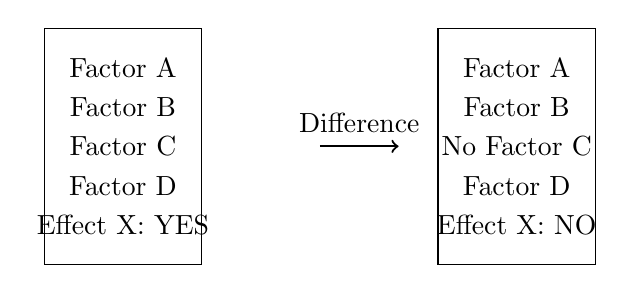
\begin{tikzpicture}
        % Two scenarios
        \draw (0,0) rectangle (2,3);
        \draw (5,0) rectangle (7,3);
        
        % Factors
        \node at (1,2.5) {Factor A};
        \node at (1,2.0) {Factor B};
        \node at (1,1.5) {Factor C};
        \node at (1,1.0) {Factor D};
        \node at (1,0.5) {Effect X: YES};
        
        \node at (6,2.5) {Factor A};
        \node at (6,2.0) {Factor B};
        \node at (6,1.5) {No Factor C};
        \node at (6,1.0) {Factor D};
        \node at (6,0.5) {Effect X: NO};
        
        % Arrow pointing to difference
        \draw[->, thick] (3.5,1.5) -- (4.5,1.5);
        \node at (4,1.8) {Difference};
    \end{tikzpicture}
    \end{center}
\end{frame}

\begin{frame}{Method of Difference Example: Dexter's Growth Serum}
	\textbf{Scenario:} Dexter wants to test whether his new growth serum causes plants to grow taller. He sets up two identical experiments.
	
	\begin{center}
		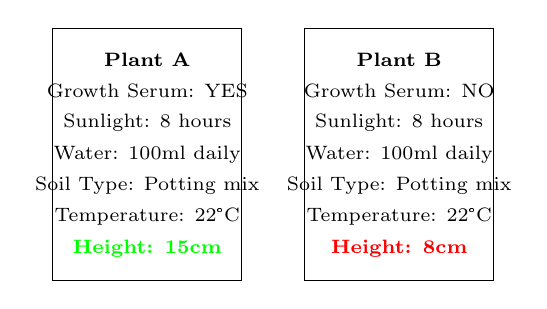
\begin{tikzpicture}[scale=0.8]
			\scriptsize
			% Experiment A
			\draw (0,0) rectangle (3,4);
			\node at (1.5,3.5) {\textbf{Plant A}};
			\node at (1.5,3) {Growth Serum: YES};
			\node at (1.5,2.5) {Sunlight: 8 hours};
			\node at (1.5,2) {Water: 100ml daily};
			\node at (1.5,1.5) {Soil Type: Potting mix};
			\node at (1.5,1) {Temperature: 22°C};
			\node at (1.5,0.5) {\textcolor{green}{\textbf{Height: 15cm}}};
			
			% Experiment B
			\draw (4,0) rectangle (7,4);
			\node at (5.5,3.5) {\textbf{Plant B}};
			\node at (5.5,3) {Growth Serum: NO};
			\node at (5.5,2.5) {Sunlight: 8 hours};
			\node at (5.5,2) {Water: 100ml daily};
			\node at (5.5,1.5) {Soil Type: Potting mix};
			\node at (5.5,1) {Temperature: 22°C};
			\node at (5.5,0.5) {\textcolor{red}{\textbf{Height: 8cm}}};
		\end{tikzpicture}
	\end{center}
	
	\textbf{Analysis:} The only difference is the growth serum, yet Plant A grew much taller.
	
	\textbf{Conclusion by Method of Difference:} The growth serum causes increased plant growth.
	
	\begin{block}{Dexter concludes:}
		"The experimental data supports my hypothesis with 93.7\% confidence!"
	\end{block}
\end{frame}


\begin{frame}{Joint Method of Agreement and Difference: Combining Approaches}
	\begin{itemize}
		\item The \textbf{Joint Method} combines the strengths of the Methods of Agreement and Difference.
		\item It looks for a factor that is present whenever the effect occurs and absent whenever the effect is absent.
		\item This method provides stronger evidence than either method alone.
		\item It reduces the likelihood of coincidental associations being mistaken for causes.
	\end{itemize}
	
	\begin{table}
		\centering
		\begin{tabular}{|c|c|c|c|c|}
			\hline
			\textbf{Case} & \textbf{Factor A} & \textbf{Factor B} & \textbf{Factor C} & \textbf{Effect X} \\
			\hline
			1 & Present & Present & Absent & Occurs \\
			2 & Present & Absent & Present & Occurs \\
			3 & Absent & Present & Present & Does Not Occur \\
			4 & Absent & Absent & Present & Does Not Occur \\
			\hline
			\multicolumn{5}{|c|}{Factor A is most likely the cause of Effect X} \\
			\hline
		\end{tabular}
	\end{table}
\end{frame}


\begin{frame}{Joint Method Example: Rick's Portal Gun Malfunctions}
	\textbf{Scenario:} Rick is investigating when his portal gun malfunctions. He needs to find what's present when it fails AND absent when it works.
	
	\begin{table}
		\scriptsize
		\centering
		\begin{tabular}{|c|c|c|c|c|c|}
			\hline
			\textbf{Test} & \textbf{Drunk} & \textbf{Morty Nearby} & \textbf{Battery Low} & \textbf{Burping} & \textbf{Malfunction?} \\
			\hline
			1 & Yes & Yes & No & Yes & YES \\
			2 & Yes & No & Yes & Yes & YES \\
			3 & No & Yes & Yes & No & NO \\
			4 & No & No & Yes & No & NO \\
			5 & Yes & No & No & Yes & YES \\
			6 & No & Yes & No & No & NO \\
			\hline
		\end{tabular}
	\end{table}
	
	\textbf{Analysis:} Being drunk is present in ALL malfunctions (tests 1, 2, 5) and absent in ALL successful uses (tests 3, 4, 6).
	
	\textbf{Conclusion by Joint Method:} Rick's drunkenness causes portal gun malfunctions.
	
	\begin{alertblock}{Rick's response:}
		"Listen Morty, *burp* the science clearly shows that alcohol actually IMPROVES my inventions... this data must be wrong, Morty!"
	\end{alertblock}
\end{frame}

\begin{frame}{Method of Residues: What's Left When Everything Else Is Explained}
    \begin{itemize}
        \item The \textbf{Method of Residues} applies when part of an effect has already been attributed to certain causes.
        \item If we subtract the known causes and their effects, what remains must be caused by the remaining factors.
        \item This method builds on existing knowledge of causal relationships.
        \item It helps identify complex causal relationships where multiple factors are involved.
    \end{itemize}
    
    \begin{alertblock}{Key Formula}
        If ABC causes XYZ, and we know A causes X and B causes Y, then C must cause Z.
    \end{alertblock}
\end{frame}

\begin{frame}{Method of Residues Example: Jimmy Neutron's Rocket Fuel}
	\scriptsize{
	\textbf{Scenario:} Jimmy's rocket achieves 1000 units of thrust, but he wants to understand what contributes to this total power.
	

	\textbf{Previous Knowledge:}
	\begin{itemize}
		\item Liquid oxygen contributes 400 units of thrust
		\item Fuel stabilizer contributes 250 units of thrust
		\item Ignition system contributes 150 units of thrust
	\end{itemize}
	
	\textbf{Current Rocket Components:}
	\begin{itemize}
		\item Liquid oxygen (400 units)
		\item Fuel stabilizer (250 units)  
		\item Ignition system (150 units)
		\item NEW: Neutronium catalyst (? units)
	\end{itemize}
	
	\textbf{Analysis by Method of Residues:}
	\begin{align}
		\text{Total thrust} &= 1000 \text{ units} \\
		\text{Known components} &= 400 + 250 + 150 = 800 \text{ units} \\
		\text{Neutronium catalyst} &= 1000 - 800 = 200 \text{ units}
	\end{align}
}
	\textbf{Conclusion:} The neutronium catalyst contributes 200 units of thrust.
	
	\begin{block}{Jimmy says:}
		"Brain blast! The neutronium catalyst accounts for exactly 20\% of our total propulsion!"
	\end{block}
\end{frame}

\begin{frame}{Method of Concomitant Variation: When Things Change Together}
    \begin{itemize}
        \item The \textbf{Method of Concomitant Variation} examines how changes in one variable relate to changes in another.
        \item If a change in Factor A consistently corresponds with a change in Effect X, they are likely causally related.
        \item This method is especially useful for factors that cannot be completely removed.
        \item It helps identify causal relationships that involve quantities rather than just presence or absence.
    \end{itemize}
    
    \begin{center}
    \begin{tikzpicture}[scale = 0.7]
        % Axes
        \draw[->] (0,0) -- (5,0) node[right] {Factor A};
        \draw[->] (0,0) -- (0,4) node[above] {Effect X};
        
        % Points
        \filldraw (0.5,0.7) circle (2pt);
        \filldraw (1.5,1.5) circle (2pt);
        \filldraw (2.5,2.3) circle (2pt);
        \filldraw (3.5,3.1) circle (2pt);
        \filldraw (4.5,3.9) circle (2pt);
        
        % Line of best fit
        \draw[red] (0.3,0.5) -- (4.7,4);
    \end{tikzpicture}
    \end{center}
\end{frame}

\begin{frame}{Applying Mill's Methods: Real-World Examples}
    \begin{itemize}
        \item Medical research often uses the Method of Difference to test whether a treatment causes improvement.
        \item Epidemiologists use the Method of Agreement to identify common factors in disease outbreaks.
        \item Social scientists apply the Method of Concomitant Variation to study how education affects income.
        \item Environmental scientists use the Joint Method to establish links between pollutants and ecosystem effects.
    \end{itemize}
    
    \begin{example}
        \textbf{Snow's Cholera Investigation (1854):} John Snow used Mill's methods to determine that contaminated water caused cholera by mapping cases and identifying a common source (the Broad Street pump).
    \end{example}
\end{frame}

\begin{frame}{The Limitations of Mill's Methods}
    \begin{itemize}
        \item Mill's methods assume we can identify all relevant factors, which is often impossible in complex situations.
        \item They don't account for probabilistic causation, where causes increase the likelihood of effects rather than guaranteeing them.
        \item The methods can be misled by coincidental correlations or hidden variables.
        \item They struggle with situations where multiple causes interact or where feedback loops exist.
    \end{itemize}
    
    \begin{alertblock}{Important Consideration}
        Mill's methods provide a useful starting point but modern science has developed more sophisticated approaches to address these limitations.
    \end{alertblock}
\end{frame}

\begin{frame}{From Philosophy to Science: The Evolution of Causal Thinking}
    \begin{itemize}
        \item Modern causal reasoning builds on Mill's methods but adds statistical analysis and experimental controls.
        \item The scientific method formalizes the process of hypothesis testing through controlled experiments.
        \item Randomized controlled trials emerged in the 20th century as the gold standard for establishing causation.
        \item Computer science and statistics have developed new mathematical tools for causal inference from data.
    \end{itemize}
    
    \begin{center}
    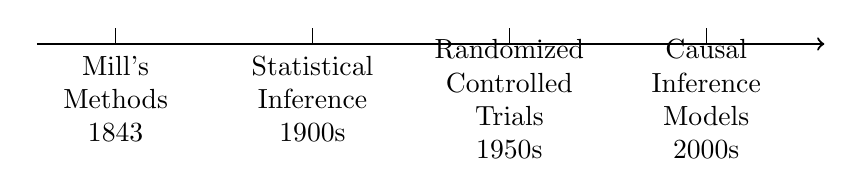
\begin{tikzpicture}
        % Timeline
        \draw[thick, ->] (0,0) -- (10,0);
        
        % Key points
        \draw (1,0) -- (1,0.2);
        \node[align=center, text width=2cm] at (1,-0.7) {Mill's Methods\\1843};
        
        \draw (3.5,0) -- (3.5,0.2);
        \node[align=center, text width=2.5cm] at (3.5,-0.7) {Statistical\\Inference\\1900s};
        
        \draw (6,0) -- (6,0.2);
        \node[align=center, text width=2.5cm] at (6,-0.7) {Randomized\\Controlled Trials\\1950s};
        
        \draw (8.5,0) -- (8.5,0.2);
        \node[align=center, text width=2.5cm] at (8.5,-0.7) {Causal\\Inference Models\\2000s};
    \end{tikzpicture}
    \end{center}
\end{frame}

\begin{frame}{Variables 101: Dependent, Independent, and Control}
    \begin{itemize}
        \item An \textbf{independent variable} is what researchers manipulate or change to see if it causes an effect.
        \item A \textbf{dependent variable} is what researchers measure to see if it was affected by the independent variable.
        \item \textbf{Control variables} are factors kept constant to ensure they don't influence the results.
        \item Understanding these variables is essential for designing experiments that can establish causation.
    \end{itemize}
    
    \begin{table}
        \centering
        \begin{tabular}{|l|p{7cm}|}
            \hline
            \textbf{Variable Type} & \textbf{Example in Plant Growth Experiment} \\
            \hline
            Independent & Amount of fertilizer applied to plants \\
            \hline
            Dependent & Height of plants after 2 weeks \\
            \hline
            Control & Type of soil, amount of water, amount of sunlight, temperature \\
            \hline
        \end{tabular}
    \end{table}
\end{frame}

\begin{frame}{Confounding Variables: The Hidden Troublemakers}
    \begin{itemize}
        \item \textbf{Confounding variables} are factors that affect both the independent and dependent variables, creating a false impression of causation.
        \item They can make it appear that A causes B when in reality C causes both A and B.
        \item Identifying and controlling for confounding variables is one of the biggest challenges in causal research.
        \item Failure to account for confounders is a common source of incorrect causal conclusions.
    \end{itemize}
    
    \begin{center}
    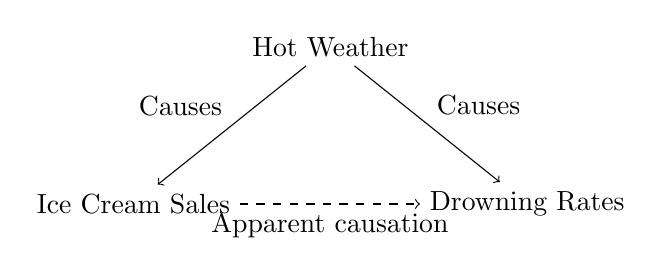
\begin{tikzpicture}
        % Nodes
        \node (A) at (0,0) {Ice Cream Sales};
        \node (B) at (5,0) {Drowning Rates};
        \node (C) at (2.5,2) {Hot Weather};
        
        % Arrows
        \draw[->, dashed] (A) -- (B) node[midway, below] {Apparent causation};
        \draw[->] (C) -- (A) node[midway, above left] {Causes};
        \draw[->] (C) -- (B) node[midway, above right] {Causes};
    \end{tikzpicture}
    \end{center}
\end{frame}

\begin{frame}{Controlled Experiments: The Gold Standard of Causal Discovery}
    \begin{itemize}
        \item A \textbf{controlled experiment} systematically manipulates one variable while keeping all others constant.
        \item The experimental group receives the treatment while the control group does not.
        \item This design isolates the effect of the independent variable on the dependent variable.
        \item Controlled experiments provide the strongest evidence for causal relationships.
    \end{itemize}
    
    \begin{block}{Key Components of a Controlled Experiment}
        \begin{itemize}
            \item Control group and experimental group(s)
            \item Random assignment of subjects
            \item Manipulation of the independent variable
            \item Measurement of the dependent variable
        \end{itemize}
    \end{block}
\end{frame}

\begin{frame}{Randomization: Why Leaving Things to Chance Makes Scientific Sense}
    \begin{itemize}
        \item \textbf{Randomization} means assigning subjects to groups by chance, not by choice or pattern.
        \item Random assignment helps distribute unknown confounding variables equally across groups.
        \item This ensures that differences between groups are likely due to the treatment, not pre-existing differences.
        \item Randomization is a crucial innovation that strengthens Mill's Method of Difference.
    \end{itemize}
    
    \begin{center}
    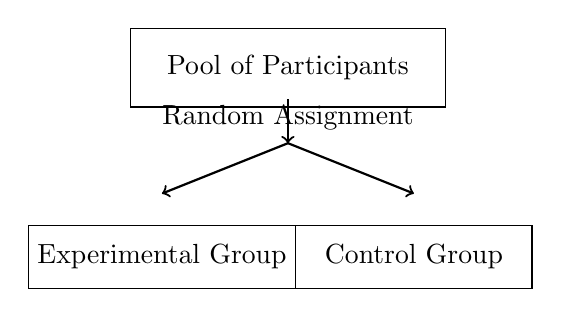
\begin{tikzpicture}[scale = 0.8]
        % Initial group
        \node[draw, rectangle, minimum width=4cm, minimum height=1cm] (pool) at (0,3) {Pool of Participants};
        
        % Arrow pointing down
        \node at (0,2.2) {Random Assignment};
        \draw[->, thick] (0,2.5) -- (0,1.8);
        
        % Split arrow
        \draw[->, thick] (0,1.8) -- (-2,1);
        \draw[->, thick] (0,1.8) -- (2,1);
        
        % Experimental and control groups
        \node[draw, rectangle, minimum width=3cm, minimum height=0.8cm] (exp) at (-2,0) {Experimental Group};
        \node[draw, rectangle, minimum width=3cm, minimum height=0.8cm] (con) at (2,0) {Control Group};
    \end{tikzpicture}
    \end{center}
\end{frame}

\begin{frame}{Sample Size and Statistical Power: Why Numbers Matter}
    \begin{itemize}
        \item \textbf{Sample size} refers to the number of subjects or observations in a study.
        \item Larger samples make it more likely to detect true effects and less likely to be misled by random variation.
        \item \textbf{Statistical power} is the ability of a study to detect an effect if one actually exists.
        \item Small studies may miss real causal relationships due to insufficient power.
    \end{itemize}
    
    \begin{table}
        \centering
        \begin{tabular}{|l|p{7cm}|}
            \hline
            \textbf{Sample Size} & \textbf{Implications} \\
            \hline
            Small ($n < 30$) & High variability, low reliability, susceptible to outliers, low power \\
            \hline
            Medium ($30 < n < 100$) & Moderate reliability, may detect large effects \\
            \hline
            Large ($n > 100$) & More reliable, can detect smaller effects, more generalizable \\
            \hline
        \end{tabular}
    \end{table}
\end{frame}

\begin{frame}{Blind and Double-Blind Studies: Removing Bias}
    \begin{itemize}
        \item In a \textbf{blind study}, participants don't know whether they're in the experimental or control group.
        \item In a \textbf{double-blind study}, neither participants nor researchers know who is in which group.
        \item Blinding prevents expectations from influencing behavior and measurements.
        \item This approach eliminates psychological biases that can create false impressions of causality.
    \end{itemize}
    
    \begin{example}
        A medication trial where patients receive either the real drug or a placebo that looks identical. Neither patients nor doctors evaluating responses know who received which treatment until after data collection is complete.
    \end{example}
\end{frame}

\begin{frame}{Placebo Effect: When Belief Causes Change}
    \begin{itemize}
        \item The \textbf{placebo effect} occurs when improvement happens because a person believes they're receiving effective treatment.
        \item This demonstrates how psychological factors can create real physiological changes.
        \item The placebo effect is a legitimate causal relationship (belief → improvement).
        \item Controlling for the placebo effect is essential in determining whether treatments have effects beyond psychological expectations.
    \end{itemize}
    
    \begin{alertblock}{Important Note}
        The placebo effect is not "fake" or "all in the mind" but a real phenomenon with measurable biological effects, including changes in brain chemistry and immune response.
    \end{alertblock}
\end{frame}

\begin{frame}{Natural Experiments: When Nature Does the Work for Us}
    \begin{itemize}
        \item \textbf{Natural experiments} occur when circumstances create comparison groups without researcher intervention.
        \item These situations allow us to study causes when deliberate experiments would be impossible or unethical.
        \item Natural experiments approximate Mill's methods in real-world settings.
        \item They provide valuable causal insights when controlled experiments aren't feasible.
    \end{itemize}
    
    \begin{example}
        After a flood in 1993, some schools in Chicago were damaged and closed, forcing students to transfer to better-performing schools. Researchers tracked these students to study the effect of school quality on academic achievement, finding significant improvements compared to similar students who stayed in their original schools.
    \end{example}
\end{frame}

\begin{frame}{Case Studies vs. Controlled Experiments: Strengths and Weaknesses}
    \begin{itemize}
        \item \textbf{Case studies} examine a single instance or small group in great depth.
        \item They provide rich detail but may not generalize to other situations.
        \item Controlled experiments offer stronger causal evidence but often sacrifice context and detail.
        \item Both approaches have complementary roles in establishing causal knowledge.
    \end{itemize}
    
    \begin{table}
        \scriptsize
        \centering
        \begin{tabular}{|l|p{3.5cm}|p{3.5cm}|}
            \hline
            \textbf{Aspect} & \textbf{Case Studies} & \textbf{Controlled Experiments} \\
            \hline
            Depth & Rich, detailed information & Limited information on many cases \\
            \hline
            Breadth & Limited to few cases & Many subjects/observations \\
            \hline
            Causal evidence & Suggestive, exploratory & Strong, confirmatory \\
            \hline
            Context & Preserved & Often removed \\
            \hline
        \end{tabular}
    \end{table}
\end{frame}

\begin{frame}{Observational Studies: Finding Patterns in the Wild}
    \begin{itemize}
        \item \textbf{Observational studies} examine existing data without manipulating variables.
        \item Researchers look for patterns and associations that suggest causal relationships.
        \item Statistical techniques help control for confounding variables after data collection.
        \item These studies are valuable when experiments are impractical but provide weaker causal evidence.
    \end{itemize}
    
    \begin{center}
    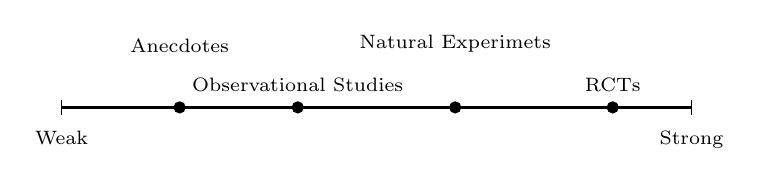
\begin{tikzpicture}[scale = 1]
        \scriptsize
        % Strength of causal evidence scale
        \draw[thick] (0,0) -- (8,0);
        \draw (0,-0.1) -- (0,0.1);
        \draw (8,-0.1) -- (8,0.1);
        \node[below] at (0,-0.2) {Weak};
        \node[below] at (8,-0.2) {Strong};
        
        % Position different study types
        \node[above] at (1.5,.6) {Anecdotes};
        \draw[fill] (1.5,0) circle (2pt);
        
        \node[above] at (3,0.1) {Observational Studies};
        \draw[fill] (3,0) circle (2pt);
        
        \node[above] at (5,.6) {Natural Experimets};
        \draw[fill] (5,0) circle (2pt);
        
        \node[above] at (7,0.1) {RCTs};
        \draw[fill] (7,0) circle (2pt);
    \end{tikzpicture}
    \end{center}
\end{frame}

\begin{frame}{Counterfactuals: Thinking About What Didn't Happen}
    \begin{itemize}
        \item A \textbf{counterfactual} is a "what if" scenario that didn't actually occur but could have.
        \item Causal claims implicitly involve counterfactuals: "If A hadn't happened, B wouldn't have happened."
        \item Controlled experiments create real-world counterfactuals through control groups.
        \item Counterfactual thinking helps us understand the logic behind causal reasoning.
    \end{itemize}
    
    \begin{block}{The Counterfactual Definition of Causation}
        Event A causes event B if and only if, had A not occurred, B would not have occurred either (assuming all else remained the same).
    \end{block}
\end{frame}

\begin{frame}{The Problem of Multiple Causes}
    \begin{itemize}
        \item Most effects in the real world have multiple causes working together.
        \item A single cause may be necessary but not sufficient to produce an effect.
        \item Multiple causal pathways may lead to the same outcome.
        \item Understanding how causes interact is essential for accurate causal reasoning.
    \end{itemize}
    
    \begin{center}
    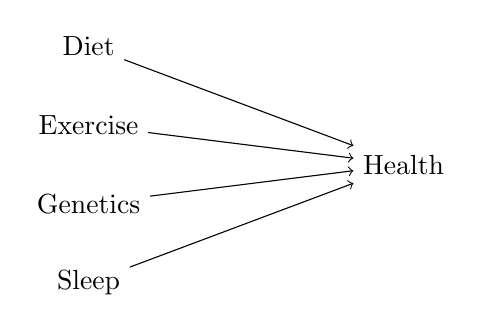
\begin{tikzpicture}
        % Causes
        \node (A) at (0,3) {Diet};
        \node (B) at (0,2) {Exercise};
        \node (C) at (0,1) {Genetics};
        \node (D) at (0,0) {Sleep};
        
        % Effect
        \node (E) at (4,1.5) {Health};
        
        % Arrows
        \draw[->] (A) -- (E);
        \draw[->] (B) -- (E);
        \draw[->] (C) -- (E);
        \draw[->] (D) -- (E);
    \end{tikzpicture}
    \end{center}
\end{frame}

\begin{frame}{When Causes Are Probabilistic, Not Deterministic}
    \begin{itemize}
        \item \textbf{Deterministic causation} means that if A occurs, B must occur.
        \item \textbf{Probabilistic causation} means that if A occurs, B becomes more likely but isn't guaranteed.
        \item Most real-world causes are probabilistic rather than deterministic.
        \item Statistical methods help us identify causes that increase the probability of effects.
    \end{itemize}
    
    \begin{example}
        Smoking causes lung cancer, but not every smoker develops lung cancer, and some non-smokers do. Smoking increases the probability of lung cancer by about 15-30 times compared to non-smokers.
    \end{example}
\end{frame}

\begin{frame}{Causal Chains: From Dominos to Complex Systems}
    \begin{itemize}
        \item \textbf{Causal chains} are sequences where one event causes another, which causes another, and so on.
        \item Understanding these chains helps identify root causes and intervention points.
        \item Longer chains have more potential breaking points, making predictions less reliable.
        \item In complex systems, causal chains may include feedback loops and interactions.
    \end{itemize}
    
    \begin{center}
    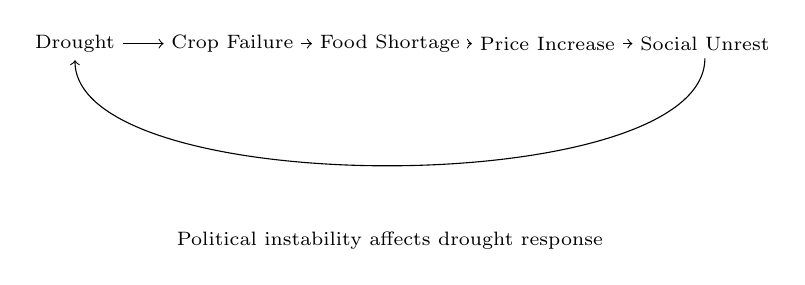
\begin{tikzpicture}
        \scriptsize
        % Basic chain
        \node (A) at (0,2) {Drought};
        \node (B) at (2,2) {Crop Failure};
        \node (C) at (4,2) {Food Shortage};
        \node (D) at (6,2) {Price Increase};
        \node (E) at (8,2) {Social Unrest};
        
        % Arrows
        \draw[->] (A) -- (B);
        \draw[->] (B) -- (C);
        \draw[->] (C) -- (D);
        \draw[->] (D) -- (E);
        
        % Feedback loop
        \draw[->] (E) .. controls (8,0) and (0,0) .. (A);
        \node at (4,-.5) {Political instability affects drought response};
    \end{tikzpicture}
    \end{center}
\end{frame}

\begin{frame}{Necessary vs. Sufficient Causes: Different Types of "Because"}
    \begin{itemize}
        \item A \textbf{necessary cause} must be present for the effect to occur (without A, no B).
        \item A \textbf{sufficient cause} guarantees the effect will occur (if A, then B).
        \item Some causes are both necessary and sufficient; others are neither.
        \item Understanding these distinctions helps clarify what we mean when we say "A causes B."
    \end{itemize}
    
    \begin{table}
        \centering
        \begin{tabular}{|l|l|l|}
            \hline
            & \textbf{Necessary} & \textbf{Not Necessary} \\
            \hline
            \textbf{Sufficient} & Oxygen for fire & Match strike for fire \\
                                & (both necessary & (sufficient but not \\
                                & and sufficient) & necessary - can use lighter) \\
            \hline
            \textbf{Not Sufficient} & Exposure to virus & Red hair for sunburn \\
                                    & for infection & (neither necessary \\
                                    & (necessary but & nor sufficient) \\
                                    & not sufficient) & \\
            \hline
        \end{tabular}
    \end{table}
\end{frame}

\begin{frame}{Simpson's Paradox: When Groups Tell Different Stories Than Individuals}
    \begin{itemize}
        \item \textbf{Simpson's Paradox} occurs when a trend appears in separate groups but disappears or reverses when the groups are combined.
        \item This paradox demonstrates how aggregating data can obscure or misrepresent causal relationships.
        \item It highlights the importance of considering subgroup differences when analyzing data.
        \item Simpson's Paradox is a warning against drawing hasty causal conclusions from statistical summaries.
    \end{itemize}
    
    \begin{center}
    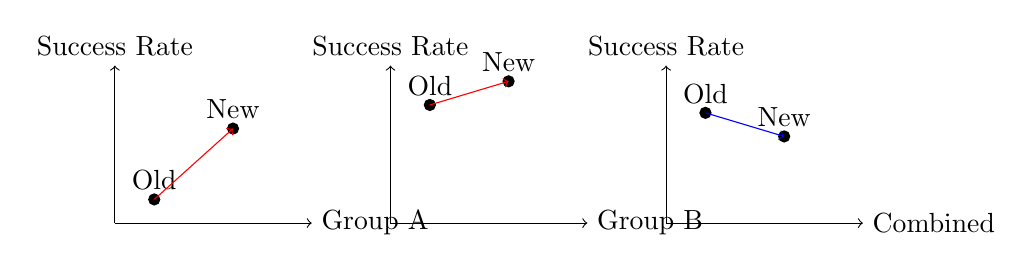
\begin{tikzpicture}
        % Axes for first graph
        \draw[->] (0,0) -- (2.5,0) node[right] {Group A};
        \draw[->] (0,0) -- (0,2) node[above] {Success Rate};
        
        % Data points and trend line
        \filldraw (0.5,0.3) circle (2pt) node[above] {Old};
        \filldraw (1.5,1.2) circle (2pt) node[above] {New};
        \draw[red, ->] (0.5,0.3) -- (1.5,1.2);
        
        % Axes for second graph
        \draw[->] (3.5,0) -- (6,0) node[right] {Group B};
        \draw[->] (3.5,0) -- (3.5,2) node[above] {Success Rate};
        
        % Data points and trend line
        \filldraw (4,1.5) circle (2pt) node[above] {Old};
        \filldraw (5,1.8) circle (2pt) node[above] {New};
        \draw[red, ->] (4,1.5) -- (5,1.8);
        
        % Axes for combined graph
        \draw[->] (7,0) -- (9.5,0) node[right] {Combined};
        \draw[->] (7,0) -- (7,2) node[above] {Success Rate};
        
        % Data points and trend line (reversed!)
        \filldraw (7.5,1.4) circle (2pt) node[above] {Old};
        \filldraw (8.5,1.1) circle (2pt) node[above] {New};
        \draw[blue, ->] (7.5,1.4) -- (8.5,1.1);
    \end{tikzpicture}
    \end{center}
\end{frame}

\begin{frame}{Common Causal Fallacies in Everyday Reasoning}
    \begin{itemize}
        \item The \textbf{post hoc fallacy} assumes that if B follows A, then A caused B (confusing sequence with causation).
        \item The \textbf{correlation fallacy} mistakes correlation for causation without considering alternative explanations.
        \item The \textbf{single-cause fallacy} assumes complex phenomena have simple, single causes.
        \item The \textbf{reversing causation fallacy} gets the direction of causality backward.
    \end{itemize}
    
    \begin{alertblock}{Warning Signs of Causal Fallacies}
        Be cautious of causal claims that:
        \begin{itemize}
            \item Involve only two variables in a complex system
            \item Are based on a few anecdotes or small samples
            \item Don't consider alternative explanations
            \item Align suspiciously well with someone's agenda
        \end{itemize}
    \end{alertblock}
\end{frame}

\begin{frame}{Critical Thinking About Causality in News and Social Media}
    \begin{itemize}
        \item News headlines often imply causation when only correlation has been established.
        \item Social media can spread causal claims without the context needed to evaluate them.
        \item Understanding research methods helps evaluate the strength of causal claims.
        \item Critical questions about sample size, confounders, and alternative explanations are essential.
    \end{itemize}
    
    \begin{example}
        \textbf{Headline}: "Study Finds Coffee Drinkers Live Longer"
        
        \textbf{Critical questions to ask}:
        Was this a controlled experiment or an observational study?
        Did researchers control for other lifestyle factors?
        Could the relationship be reversed (do healthier people drink more coffee)?
        How large was the sample size and how significant was the effect?
    \end{example}
\end{frame}

\begin{frame}{Ethics in Causal Research: When We Can't Do Certain Experiments}
    \begin{itemize}
        \item Many important causal questions cannot be studied through controlled experiments due to ethical constraints.
        \item It would be unethical to deliberately expose people to potential harms, even for knowledge.
        \item Researchers must use alternative methods like natural experiments and observational studies.
        \item Ethical considerations shape how we acquire causal knowledge about human behavior and health.
    \end{itemize}
    
    \begin{block}{Examples of Ethical Boundaries}
        We cannot ethically conduct experiments to determine:
        \begin{itemize}
            \item Whether smoking causes cancer by assigning people to smoke
            \item The effects of abuse or neglect on children's development
            \item Long-term effects of illegal drugs by giving them to participants
            \item How pollution affects health by deliberately exposing communities
        \end{itemize}
    \end{block}
\end{frame}

\begin{frame}{Modern Causal Inference: Beyond Mill's Methods}
    \begin{itemize}
        \item \textbf{Causal inference} is the modern field that develops mathematical and statistical tools for establishing causation.
        \item \textbf{Directed Acyclic Graphs (DAGs)} provide visual representations of causal relationships in complex systems.
        \item \textbf{Propensity score matching} helps simulate experimental conditions with observational data.
        \item \textbf{Instrumental variables} exploit natural randomization to establish causal effects.
    \end{itemize}
    
    \begin{center}
    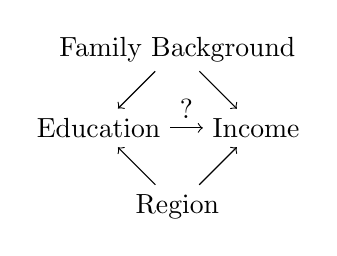
\begin{tikzpicture}
        % Simple DAG example
        \node (A) at (0,1) {Education};
        \node (B) at (2,1) {Income};
        \node (C) at (1,2) {Family Background};
        \node (D) at (1,0) {Region};
        
        % Arrows
        \draw[->] (A) -- (B) node[midway, above] {?};
        \draw[->] (C) -- (A);
        \draw[->] (C) -- (B);
        \draw[->] (D) -- (A);
        \draw[->] (D) -- (B);
    \end{tikzpicture}
    \end{center}
\end{frame}

\begin{frame}{Data Science and Causality: New Frontiers}
    \begin{itemize}
        \item Big data and machine learning are creating new opportunities and challenges for causal reasoning.
        \item Correlation-focused algorithms can find patterns but struggle to establish causation.
        \item \textbf{Causal machine learning} combines traditional experimental design with modern computational methods.
        \item These approaches help us move from "what happened" to understanding "why it happened."
    \end{itemize}
    
    \begin{alertblock}{Important Distinction}
        "Machine learning provides the power to predict but not necessarily to understand. Causal reasoning provides the understanding necessary for meaningful intervention."
        
        – Judea Pearl, Computer Scientist and Causality Researcher
    \end{alertblock}
\end{frame}

\begin{frame}{Causality in Your Life: Making Better Decisions}
    \begin{itemize}
        \item Understanding causal reasoning helps you evaluate claims in media, advertising, and politics.
        \item Causal thinking improves personal decision-making by distinguishing between correlation and causation.
        \item Seeking evidence for causal claims protects against manipulation and misinformation.
        \item The principles of causal inference apply to everything from personal health choices to policy decisions.
    \end{itemize}
    
    \begin{block}{Summary: From Mill to Modern Experiments}
        \scriptsize
        \begin{itemize}
            \item Mill's methods provide a foundation for systematic causal reasoning
            \item Controlled experiments strengthen causal evidence through randomization and controls
            \item Understanding causal complexity helps us navigate an increasingly complicated world
            \item Critical thinking about causality is an essential skill for informed citizenship
        \end{itemize}
    \end{block}
\end{frame}

% Additional frames for references or questions could be added here

\end{document}

\end{document}